% Created 2019-03-11 Mon 17:24
\documentclass[11pt]{article}
\usepackage[utf8]{inputenc}
\usepackage[T1]{fontenc}
\usepackage{fixltx2e}
\usepackage{graphicx}
\usepackage{longtable}
\usepackage{float}
\usepackage{wrapfig}
\usepackage{rotating}
\usepackage[normalem]{ulem}
\usepackage{amsmath}
\usepackage{textcomp}
\usepackage{marvosym}
\usepackage{wasysym}
\usepackage{amssymb}
\usepackage{hyperref}
\tolerance=1000
\usepackage{minted}
\usepackage{amsthm}
\usepackage[margin=1.0in]{geometry}
\setlength{\parindent}{0pt}
\setlength{\parskip}{\baselineskip}
\author{Thomas Alford}
\date{\today}
\title{Ph21 Problem Set 6}
\hypersetup{
  pdfkeywords={},
  pdfsubject={},
  pdfcreator={Emacs 25.2.1 (Org mode 8.2.10)}}
\begin{document}

\maketitle
\section*{1}
\label{sec-1}
\subsection*{Imports}
\label{sec-1-1}
\begin{minted}[frame=lines,fontsize=\scriptsize]{python}
import numpy as np
import matplotlib.pyplot as plt
%matplotlib inline
\end{minted}

\subsection*{Principle Component Analysis}
\label{sec-1-2}

\begin{minted}[frame=lines,fontsize=\scriptsize]{python}
def PCA(X):
    # here X is an m x n matrix which contains m measurement types and n samples
    Xprime = np.array([x - np.mean(x) for x in X])
    covariance = np.cov(Xprime)
    eigenvals, eigenvecs = np.linalg.eig(covariance)
    return eigenvals, eigenvecs
\end{minted}

\section*{2}
\label{sec-2}
\subsection*{Simulated Data Set (2d)}
\label{sec-2-1}

Here we'll create a data set which has x linearly dependent of y but with a
random amount of Gaussian noise involved:

\begin{minted}[frame=lines,fontsize=\scriptsize]{python}
def create_2d_data(n, mu, sigma, noise_sigma):
    y_vals = np.random.normal(mu, sigma, n)
    # create a linear relation with noise
    x_vals = 2 * y_vals + np.random.normal(0, noise_sigma, n) 
    return x_vals, y_vals
\end{minted}


\begin{minted}[frame=lines,fontsize=\scriptsize]{python}
data = create_2d_data(100, 2, 2, 1)
evals, evecs = PCA(data)
\end{minted}


\begin{minted}[frame=lines,fontsize=\scriptsize]{python}
plt.scatter(data[0], data[1], s=1)
origin = (np.mean(data[0]), np.mean(data[1]))
# multiply by sqrt(lambda)
V = evecs.T * np.array(2 * [np.sqrt(evals)]).T
plt.quiver(*origin, V[:,0], V[:,1], color=['g', 'r'], 
           angles='xy', scale=1, scale_units='xy')
plt.xlabel('x')
plt.ylabel('y')
plt.show()
\end{minted}

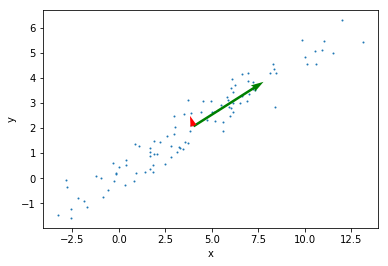
\includegraphics[width=.9\linewidth]{./obipy-resources/692met.png}

\begin{minted}[frame=lines,fontsize=\scriptsize]{python}
print('eiegnvals = ', evals)
print('eiegnvecs = ', evecs)
\end{minted}

\begin{verbatim}
eiegnvals =  [24.43196754  0.21322486]
eiegnvecs =  [[ 0.90075419 -0.43432923]
 [ 0.43432923  0.90075419]]
\end{verbatim}

Here these values make sense, as x is very dependent on y here, and y is not
dependent on x at all (the noise makes it so that this dependence isn't
perfect, however).


\section*{3}
\label{sec-3}
\subsection*{Higher Dimensional Data Set}
\label{sec-3-1}

Here now we'll simulate a higher dimensional dataset where each element is
slightly dependent on the other elements. We'll choose 5 dimensions here.

\begin{minted}[frame=lines,fontsize=\scriptsize]{python}
def create_5d_data(n, y_mu, y_sigma, noise_sigma):
    y_vals = np.random.normal(y_mu, y_sigma, n)
    # create a linear relation with noise
    x_vals = 2 * y_vals + np.random.normal(0, noise_sigma, n) 
    z_vals = .5 * y_vals - .7 * x_vals + np.random.normal(0, noise_sigma, n)
    w_vals = np.random.normal(y_mu + 10, y_sigma, n)
    v_vals = -.3 * w_vals + 1.5 * z_vals + np.random.normal(0, noise_sigma, n)
    return v_vals, w_vals, x_vals, y_vals, z_vals
\end{minted}


\begin{minted}[frame=lines,fontsize=\scriptsize]{python}
data_5d = create_5d_data(100, 2, 2, 1)
evals_5d, evecs_5d = PCA(data_5d)
\end{minted}


\begin{minted}[frame=lines,fontsize=\scriptsize]{python}
list(evals_5d)
\end{minted}

\begin{verbatim}
  [33.47792791833488,
  5.314471270308553,
  2.1399570795143403,
  0.24691964621245038,
  0.1475084147204272]
\end{verbatim}

\begin{minted}[frame=lines,fontsize=\scriptsize]{python}
evecs_5d.T
\end{minted}

\begin{verbatim}
  array([[-0.55094958,  0.02537261,  0.68413801,  0.31660392, -0.35711054],
  [ 0.33225504, -0.89601528,  0.25838908,  0.1358716 ,  0.03920705],
  [ 0.62138085,  0.43289284,  0.50514353,  0.2891418 ,  0.29616998],
  [-0.4418413 , -0.09446484, -0.01958823,  0.24750149,  0.8568617 ],
  [-0.06872597, -0.01389335,  0.45786088, -0.85816135,  0.22137352]])
\end{verbatim}

This values make sense for us. $v$ contains data about every single variable,
since it is a linear combination of $w$ and $z$, which is then a linear
combination of $x$ and $y$. Since $x$ is also dependent on $y$, this makes $z$,
$x$, and $y$ all very redundant variables, which is why their components are so
low. $w$ is the second-highest due to the fact that the only variable
dependent on it is $v$.
% Emacs 25.2.1 (Org mode 8.2.10)
\end{document}
